\begin{figure}[h]
	\centering
	\captionsetup[subfigure]{labelformat=empty}
	%c1
	\begin{subfigure}[t]{.1\textwidth}
		\centering
		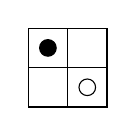
\begin{tikzpicture}[x=1cm]
			\draw (0,0)--(1,0)--(1,1)--(0,1)--cycle;
			\draw (.5,0)--(.5,.5)--(.5,1);
			\draw (0,.5)--(.5,.5)--(1,.5);
			\draw (.75,.25) circle (3pt);
			\filldraw (.25,.75) circle (3pt);
		\end{tikzpicture}
		\caption{$c_{1}$}
	\end{subfigure}%
	%c2
	\begin{subfigure}[t]{.1\textwidth}
		\centering
		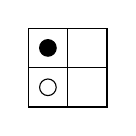
\begin{tikzpicture}[x=1cm]
			\draw (0,0)--(1,0)--(1,1)--(0,1)--cycle;
			\draw (.5,0)--(.5,.5)--(.5,1);
			\draw (0,.5)--(.5,.5)--(1,.5);
			\draw (.25,.25) circle (3pt);
			\filldraw (.25,.75) circle (3pt);
		\end{tikzpicture}
		\caption{$c_{2}$}
	\end{subfigure}%
	%c3
	\begin{subfigure}[t]{.1\textwidth}
		\centering
		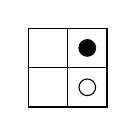
\begin{tikzpicture}[x=1cm]
			\draw (0,0)--(1,0)--(1,1)--(0,1)--cycle;
			\draw (.5,0)--(.5,.5)--(.5,1);
			\draw (0,.5)--(.5,.5)--(1,.5);
			\draw (.75,.25) circle (3pt);
			\filldraw (.75,.75) circle (3pt);
		\end{tikzpicture}
		\caption{$c_{3}$}
	\end{subfigure}%
	%c4
	\begin{subfigure}[t]{.1\textwidth}
		\centering
		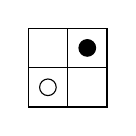
\begin{tikzpicture}[x=1cm]
			\draw (0,0)--(1,0)--(1,1)--(0,1)--cycle;
			\draw (.5,0)--(.5,.5)--(.5,1);
			\draw (0,.5)--(.5,.5)--(1,.5);
			\draw (.25,.25) circle (3pt);
			\filldraw (.75,.75) circle (3pt);
		\end{tikzpicture}
		\caption{$c_{4}$}
	\end{subfigure}%
	%c5
	\begin{subfigure}[t]{.1\textwidth}
		\centering
		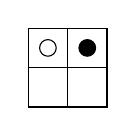
\begin{tikzpicture}[x=1cm]
			\draw (0,0)--(1,0)--(1,1)--(0,1)--cycle;
			\draw (.5,0)--(.5,.5)--(.5,1);
			\draw (0,.5)--(.5,.5)--(1,.5);
			\draw (.25,.75) circle (3pt);
			\filldraw (.75,.75) circle (3pt);
		\end{tikzpicture}
		\caption{$c_{5}$}
	\end{subfigure}%
	%c6
	\begin{subfigure}[t]{.1\textwidth}
		\centering
		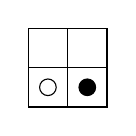
\begin{tikzpicture}[x=1cm]
			\draw (0,0)--(1,0)--(1,1)--(0,1)--cycle;
			\draw (.5,0)--(.5,.5)--(.5,1);
			\draw (0,.5)--(.5,.5)--(1,.5);
			\draw (.25,.25) circle (3pt);
			\filldraw (.75,.25) circle (3pt);
		\end{tikzpicture}
		\caption{$c_{6}$}
	\end{subfigure}
	
	%c7
	\begin{subfigure}[t]{.1\textwidth}
		\centering
		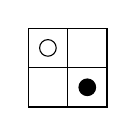
\begin{tikzpicture}[x=1cm]
			\draw (0,0)--(1,0)--(1,1)--(0,1)--cycle;
			\draw (.5,0)--(.5,.5)--(.5,1);
			\draw (0,.5)--(.5,.5)--(1,.5);
			\draw (.25,.75) circle (3pt);
			\filldraw (.75,.25) circle (3pt);
		\end{tikzpicture}
		\caption{$c_{7}$}
	\end{subfigure}%
	%c8
	\begin{subfigure}[t]{.1\textwidth}
		\centering
		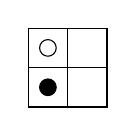
\begin{tikzpicture}[x=1cm]
			\draw (0,0)--(1,0)--(1,1)--(0,1)--cycle;
			\draw (.5,0)--(.5,.5)--(.5,1);
			\draw (0,.5)--(.5,.5)--(1,.5);
			\draw (.25,.75) circle (3pt);
			\filldraw (.25,.25) circle (3pt);
		\end{tikzpicture}
		\caption{$c_{8}$}
	\end{subfigure}%
	%c9
	\begin{subfigure}[t]{.1\textwidth}
		\centering
		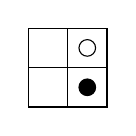
\begin{tikzpicture}[x=1cm]
			\draw (0,0)--(1,0)--(1,1)--(0,1)--cycle;
			\draw (.5,0)--(.5,.5)--(.5,1);
			\draw (0,.5)--(.5,.5)--(1,.5);
			\draw (.75,.75) circle (3pt);
			\filldraw (.75,.25) circle (3pt);
		\end{tikzpicture}
		\caption{$c_{9}$}
	\end{subfigure}%
	%c10
	\begin{subfigure}[t]{.1\textwidth}
		\centering
		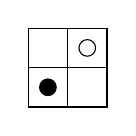
\begin{tikzpicture}[x=1cm]
			\draw (0,0)--(1,0)--(1,1)--(0,1)--cycle;
			\draw (.5,0)--(.5,.5)--(.5,1);
			\draw (0,.5)--(.5,.5)--(1,.5);
			\draw (.75,.75) circle (3pt);
			\filldraw (.25,.25) circle (3pt);
		\end{tikzpicture}
		\caption{$c_{10}$}
	\end{subfigure}%
	%c11
	\begin{subfigure}[t]{.1\textwidth}
		\centering
		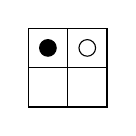
\begin{tikzpicture}[x=1cm]
			\draw (0,0)--(1,0)--(1,1)--(0,1)--cycle;
			\draw (.5,0)--(.5,.5)--(.5,1);
			\draw (0,.5)--(.5,.5)--(1,.5);
			\draw (.75,.75) circle (3pt);
			\filldraw (.25,.75) circle (3pt);
		\end{tikzpicture}
		\caption{$c_{11}$}
	\end{subfigure}%
	%c12
	\begin{subfigure}[t]{.1\textwidth}
		\centering
		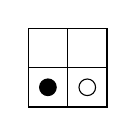
\begin{tikzpicture}[x=1cm]
			\draw (0,0)--(1,0)--(1,1)--(0,1)--cycle;
			\draw (.5,0)--(.5,.5)--(.5,1);
			\draw (0,.5)--(.5,.5)--(1,.5);
			\draw (.75,.25) circle (3pt);
			\filldraw (.25,.25) circle (3pt);
		\end{tikzpicture}
		\caption{$c_{12}$}
	\end{subfigure}
	\caption{Twelve configurations}
\end{figure}